\documentclass[12pt, a4paper]{article}
\usepackage[utf8]{inputenc}
\usepackage[italian]{babel}
\usepackage{graphicx} 
\usepackage{amsmath}
\usepackage{float}
\usepackage{hyperref}
\usepackage[a4paper, margin=2.0cm]{geometry}
\usepackage{listings}
\usepackage{url}
\usepackage{tikz}
\usetikzlibrary{positioning, arrows.meta}

\title{Manuale Tecnico}
\author{Niccolò Jacopo Alt, Alessia Gerti, Mateo Soldo, Davide Vignati}
\date{20/07/2026}

\newpage
\begin{document}
\newpage

\maketitle
\newpage
\tableofcontents
\newpage
\maketitle

\section{Introduzione}
Il manuale tecnico nasce con l'obiettivo di descrivere nel dettaglio le scelte progetturali, architetturali e tecnologiche adottate nello sviluppo del sistema \textbf{CineMax}. 

La documentazione si focalizza sull'estensione dell'applicazione verso un'architettura \textit{Client} e \textit{Server} multithread e sull'interrogazione di una base di dati relazionale per la persistenza delle informazioni. 

All'interno della documentazione viene fornita una panoramica esaustiva sugli strumenti, sulle librerie esterne e sui driver di connessione (JDBC) utilizzati. Vengono illustrati i principi che hanno guidato la realizzazione del software con riferimento ai design pattern orientati agli oggetti, alle strutture dati impiegate e alla gestione degli accessi concorrenti alle risorse condivise.

Un ampio spazio è dedicato alla formalizzazione dei modelli grafici, sia a livello logico-funzionale del codice tramite diagrammi UML (\textit{Unified Modeling Language}), sia a livello della persistenza dei dati attraverso la modellazione concettuale ER (\textit{Entity-Relationship}) e la derivazione dello schema relazionale normalizzato. 

Infine, il manuale tecnico serve per chiarire la logica architetturale e transazionale alla base del progetto, facilitandone così la comprensione, la manutenibilità e l'eventuale ripresa futura, evidenziando le potenzialità di un approccio modulare e scalabile che permette all'applicazione di crescere ed evolversi senza perdere coerenza interna.


\section{Installazione e configurazione dell'ambiente}
Per poter configurare l'ambiente di sviluppo, compilare ed eseguire il sistema \textbf{CineMax} è necessario installare e configurare i componenti software descritti di seguito. Le procedure fanno riferimento a un'installazione centralizzata su una singola macchina di sviluppo (host locale), sulla quale risiederanno sia l'ambiente di runtime che la base di dati.

\subsection{Installazione dei componenti software}

\subsubsection{Java Development Kit (JDK 25 LTS)}
Il sistema richiede la presenza della JDK per l'esecuzione e lo sviluppo dell'applicazione. Si raccomanda l'utilizzo di una versione LTS (\textbf{Long-Term-Support}) stabile, nello specifico \textbf{JDK 25}, per garantire la piena compatibilità con i driver JDBC di PostgreSQL e il corretto supporto alle funzionalità del linguaggio.

Per procedere, è necessario collegarsi al sito ufficiale Oracle nella sezione ``Java Downloads'' e scaricare il pacchetto idoneo all'architettura del proprio sistema operativo (Windows, Linux e macOS).

\begin{figure}[H]
    \centering
    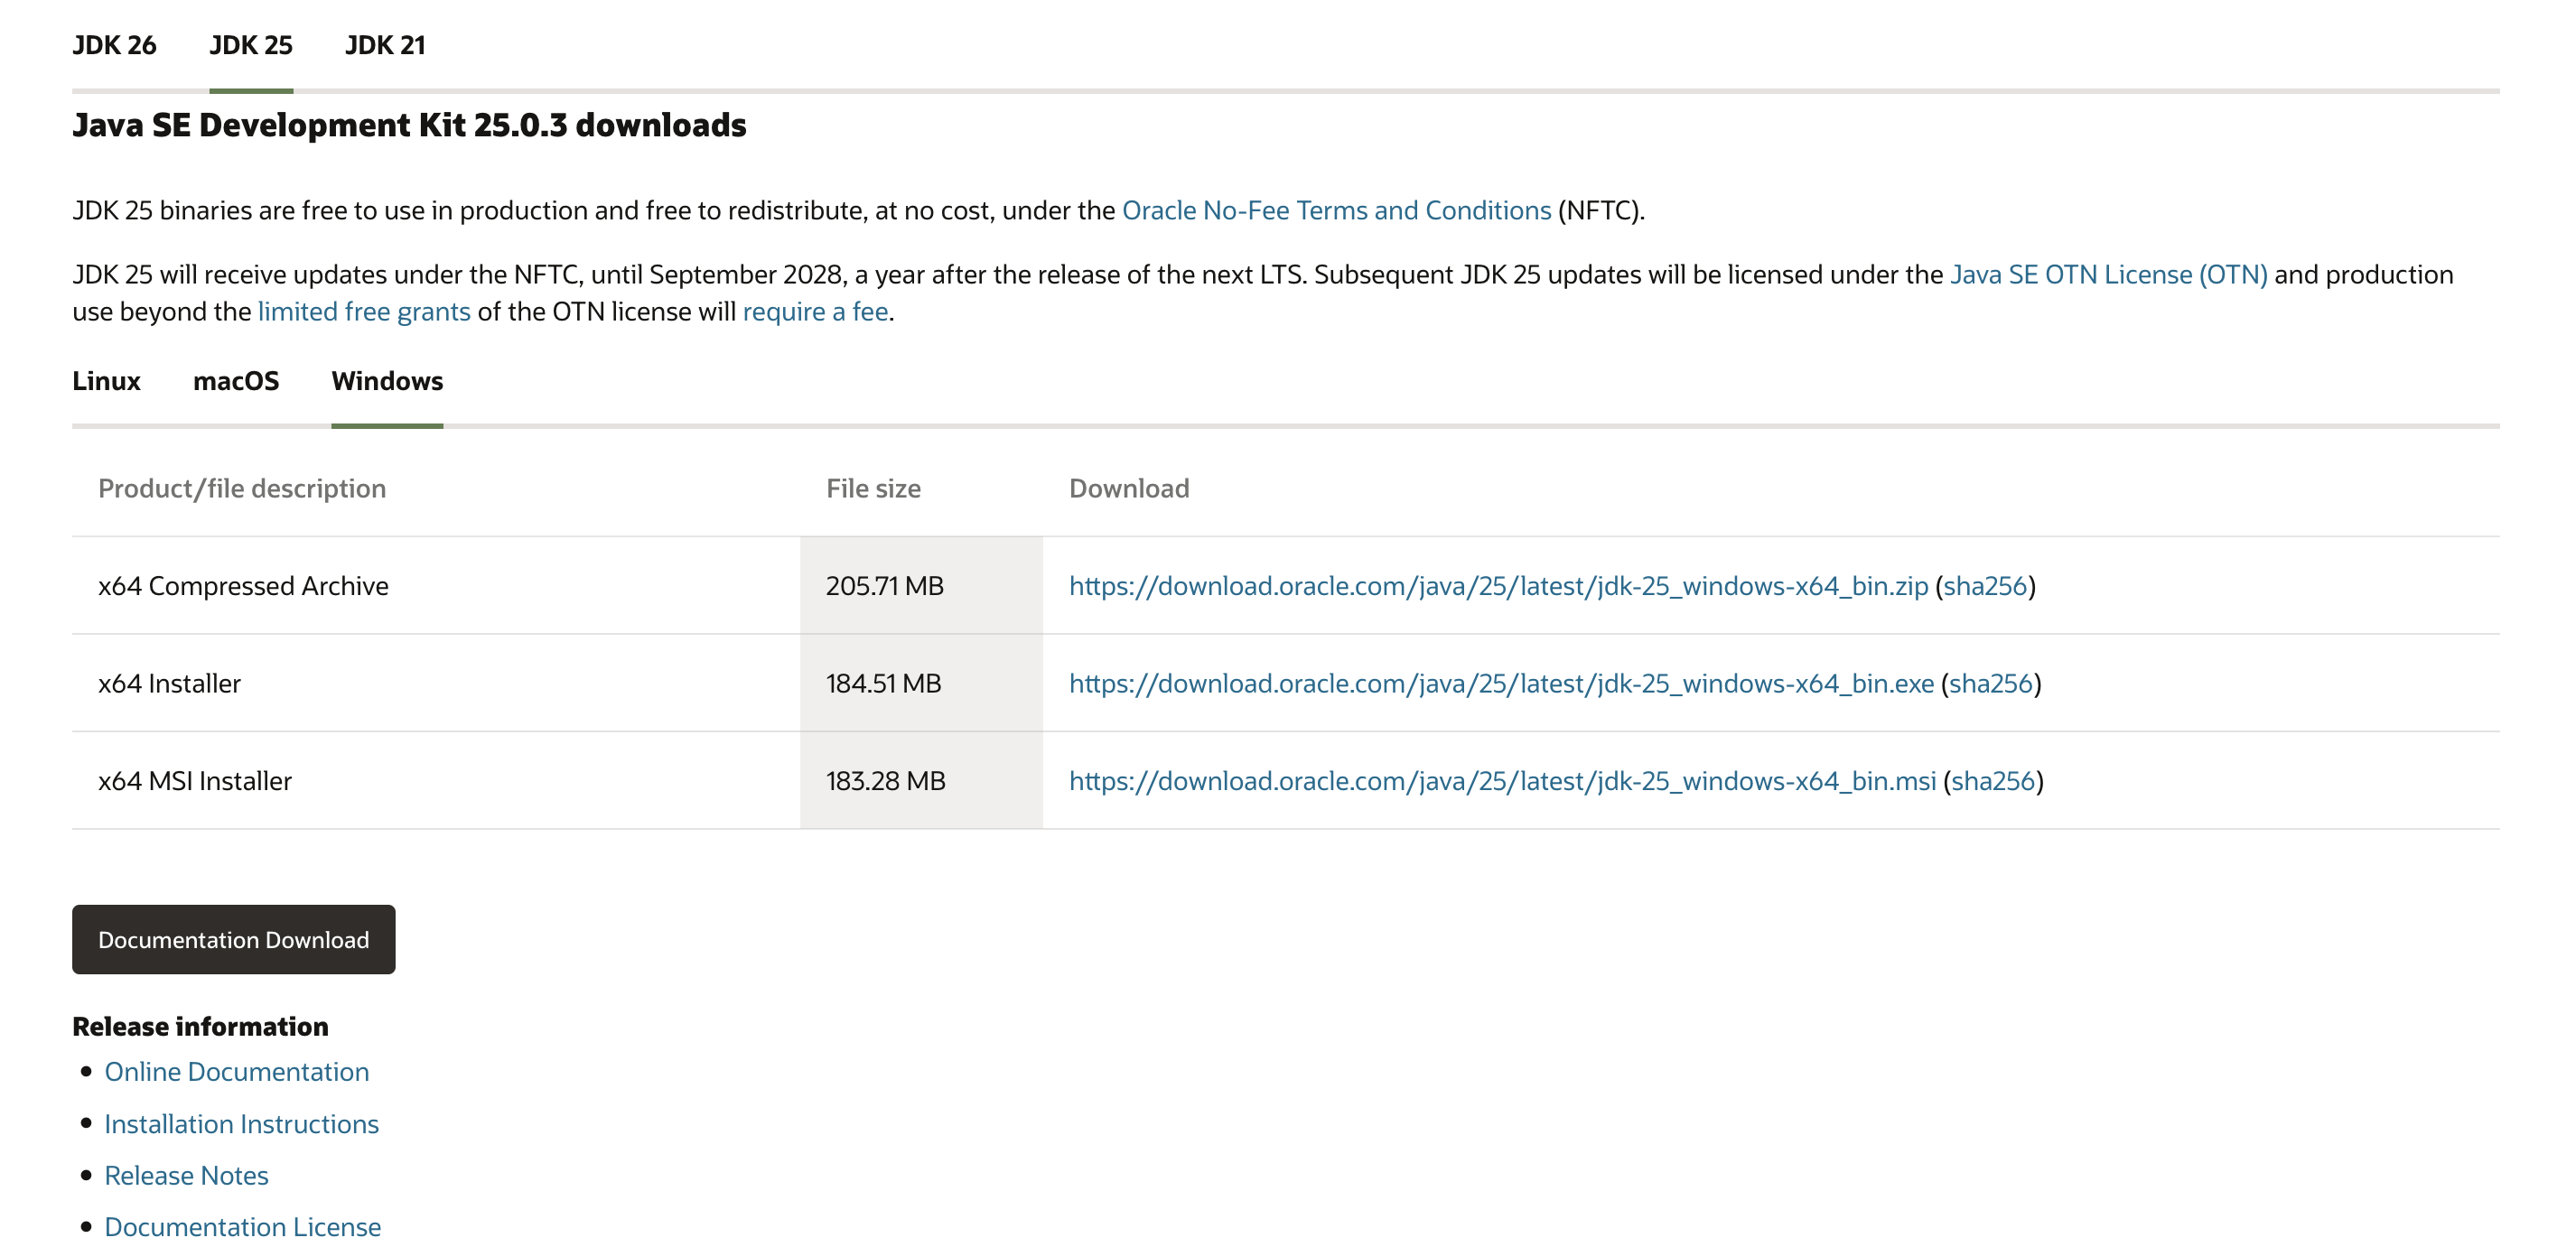
\includegraphics[width=1.0\linewidth]{oracle.png} 
    \caption{Sito ufficiale Oracle per il download di Java 25}
    \label{fig:oracle}
\end{figure}

\textbf{Nota per gli utenti macOS:} La versione ``ARM64 DMG Installer'' è dedicata ai Mac con processori Apple Silicon (M1, M2, M3, ecc.), mentre la versione ``x64 DMG Installer'' è destinata ai Mac dotati di processore Intel.\\
Dopo aver completato l'installazione guidata, è necessario configurare le variabili d'ambiente per consentire l'esecuzione corretta dei comandi Java da terminale.

\paragraph{Windows} 
Accedere al pannello ``Variabili d'ambiente'' dal menu Start. Creare una nuova variabile di sistema denominata \texttt{JAVA\_HOME} che punti alla cartella radice della JDK installata (es. \texttt{C:\textbackslash Program Files\textbackslash Java\textbackslash jdk-25}). Successivamente, selezionare la variabile \texttt{Path}, cliccare su ``Modifica'' e aggiungere il percorso della cartella bin: \texttt{\%JAVA\_HOME\%\textbackslash bin}.

\paragraph{Linux}
Eseguire l'estrazione dell'archivio compresso nella directory di sistema:
\begin{verbatim}
sudo mkdir -p /usr/local/java
sudo tar -xzvf jdk-25_linux-x64_bin.tar.gz -C /usr/local/java/
\end{verbatim}
Modificare il file di configurazione globale del sistema tramite il comando \texttt{sudo nano /etc/profile} aggiungendo le seguenti righe:
\begin{verbatim}
export JAVA_HOME=/usr/local/java/jdk-25
export PATH=$PATH:$JAVA_HOME/bin
\end{verbatim}
Applicare le modifiche digitando: \texttt{source /etc/profile}.

\paragraph{macOS}
Modificare il file di configurazione della shell zsh tramite \texttt{nano ~/.zshrc} inserendo:
\begin{verbatim}
export JAVA_HOME="/Library/Java/JavaVirtualMachines/jdk-25.jdk/Contents/Home"
export PATH="$PATH:$JAVA_HOME/bin"
\end{verbatim}

Salvare premendo \texttt{Ctrl+O}, confermare con \texttt{Invio} e uscire con \texttt{Ctrl+X}. Rendere effettive le modifiche con il comando: \texttt{source ~/.zshrc}.\\
Verificare la corretta installazione digitando da terminale: \texttt{java -version}.

\subsection{Apache Maven}
Il progetto utilizza Apache Maven per la gestione del ciclo di vita del software, l'automazione della build e la risoluzione delle dipendenze (come il driver JDBC) definite nel file \texttt{pom.xml}.

\begin{figure}[H]
    \centering
 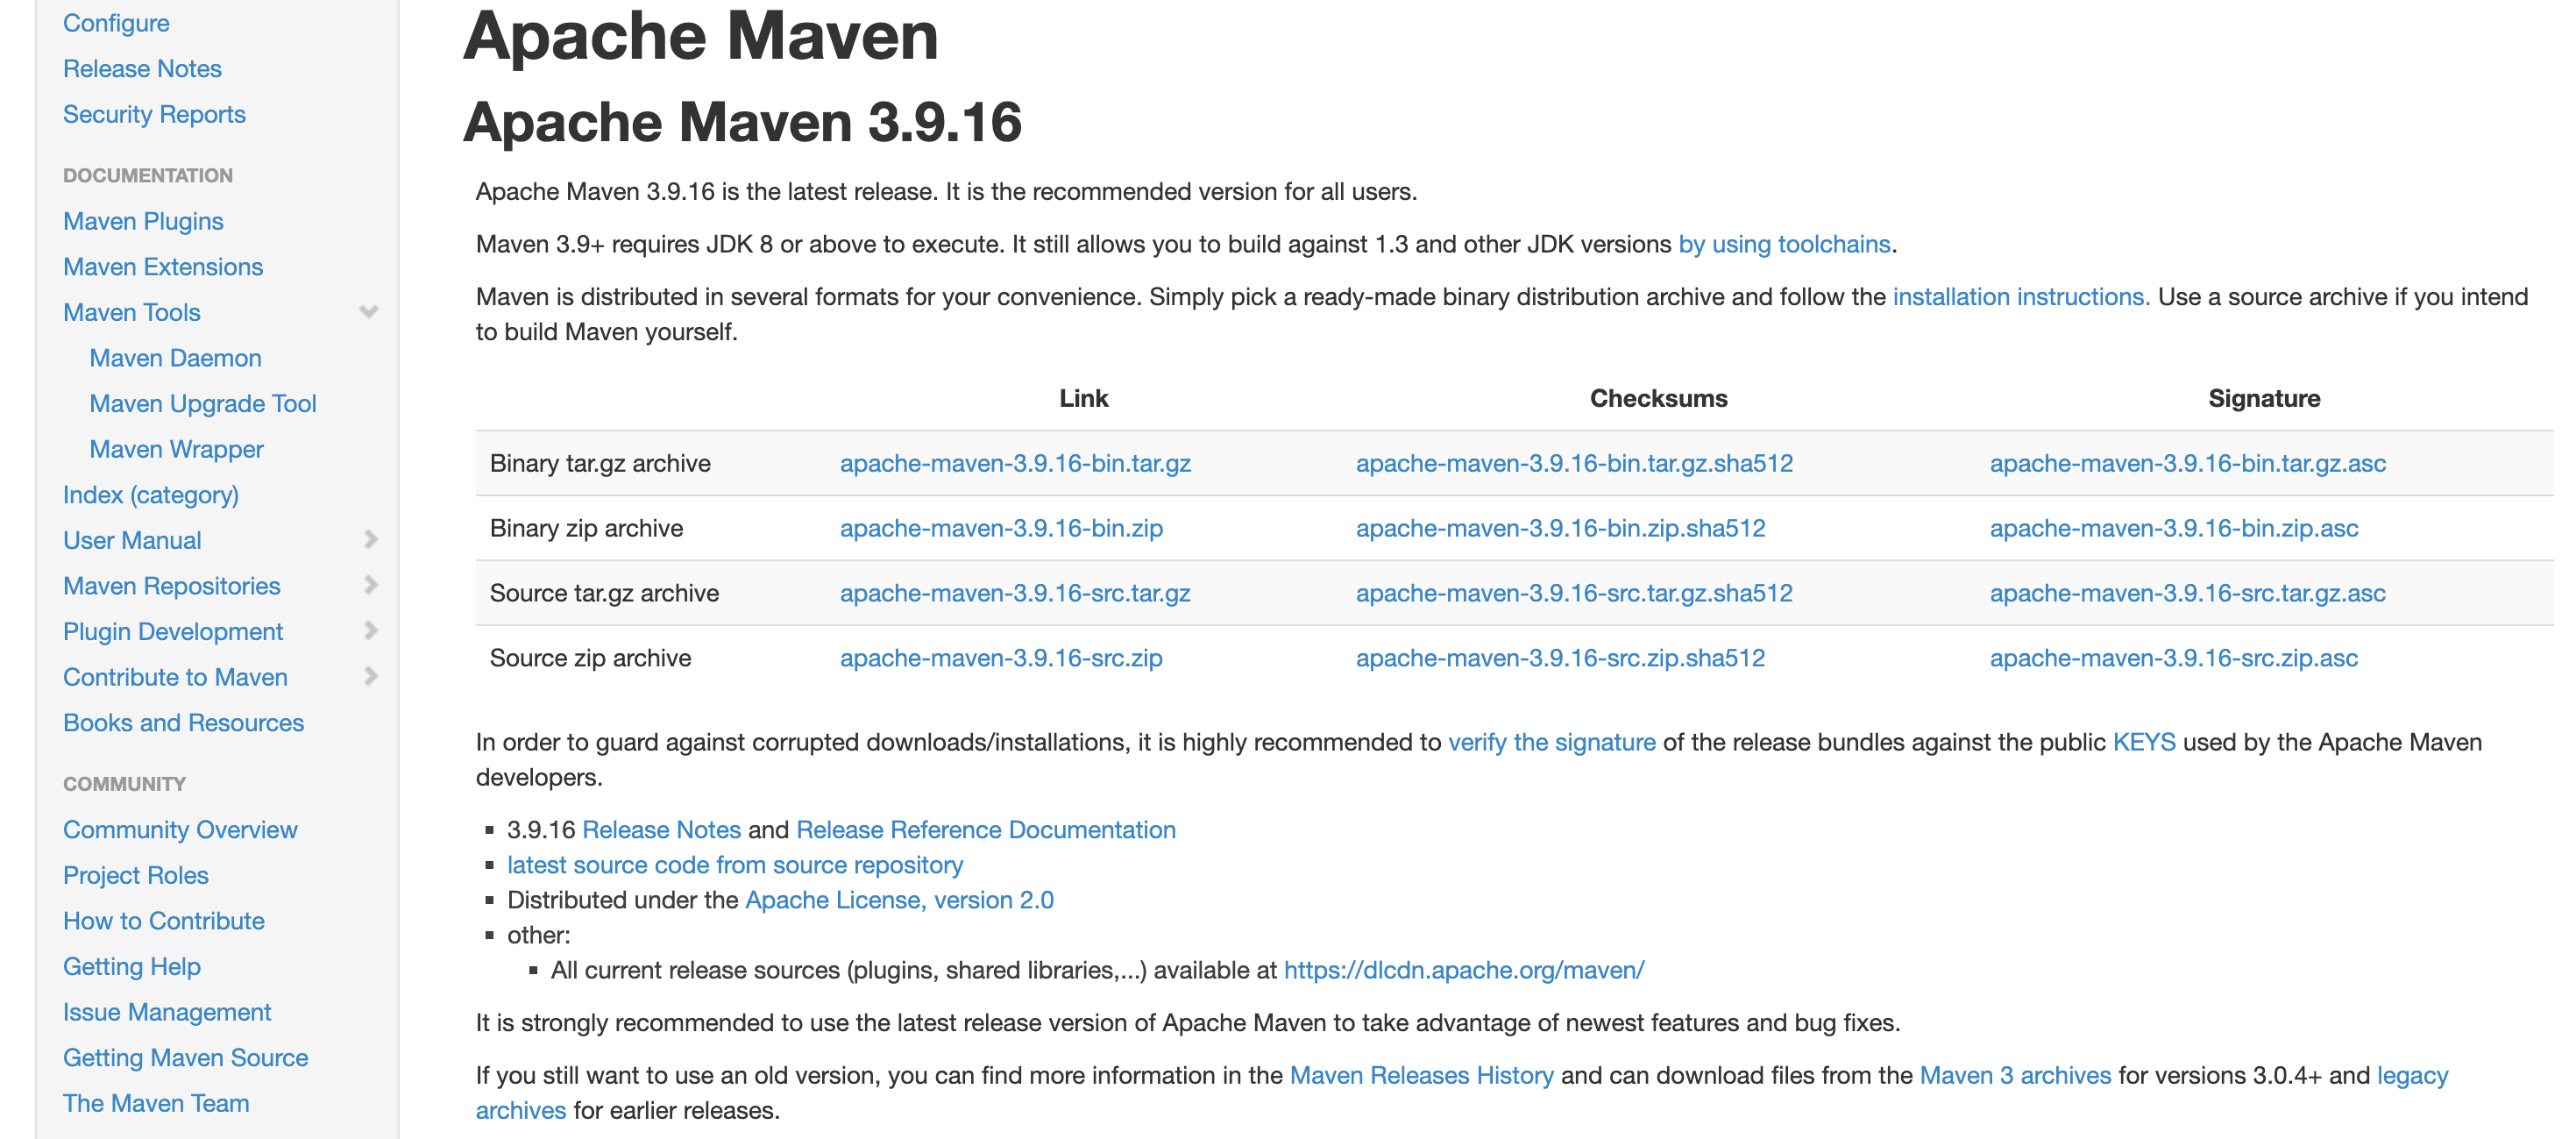
\includegraphics[width=1.0\linewidth]{maven.png}
    \caption{Sito ufficiale Apache Maven}
    \label{fig:maven}
\end{figure}

\paragraph{Windows}
Scaricare il ``Binary zip archive'' dal sito ufficiale. Estrarre il contenuto in una cartella permanente (es. \texttt{C:\textbackslash apache-maven-3.9.6}). Nel pannello delle variabili d'ambiente, modificare la variabile di sistema \texttt{Path} inserendo il percorso della cartella bin di Maven (es. \texttt{C:\textbackslash apache-maven-3.9.6\textbackslash bin}).

\paragraph{Linux}
Sulle distribuzioni basate su Debian/Ubuntu, l'aggiunta avviene tramite il gestore di pacchetti Apt:
\begin{verbatim}
sudo apt update
sudo apt install maven
\end{verbatim}

\paragraph{macOS}
L'installazione consigliata avviene tramite l'ausilio del package manager Homebrew:
\begin{verbatim}
brew install maven
\end{verbatim}
Verificare l'installazione digitando da terminale: \texttt{mvn -version}.

\subsection{PostgreSQL RDBMS}
Per garantire la persistenza a lungo termine dei dati relativi a utenti, film, proiezioni e prenotazioni del cinema, il sistema CineMax richiede un'istanza attiva del database relazionale PostgreSQL (versione 15 o successiva). Nell'architettura ad host singolo, il server del database viene eseguito ed ospitato localmente sulla stessa macchina su cui viene avviata l'applicazione.

\subsubsection{Installazione}
L'installazione e la prima inizializzazione del sistema di gestione di basi di dati variano a seconda del sistema operativo in uso:
\begin{itemize}
    \item \textbf{Windows / macOS}: È necessario scaricare l'installer grafico dal sito ufficiale ed eseguire il setup guidato. Durante il processo, occorre definire la password per l'utente amministratore di default (\texttt{postgres}) e mantenere la porta di ascolto standard \texttt{5432}. Si raccomanda caldamente di includere l'installazione di \textbf{pgAdmin 4} (già integrato nell'installer) per usufruire di un'interfaccia grafica intuitiva atta alla gestione visuale della base dati.
    \item \textbf{Linux (Debian/Ubuntu)}: L'installazione avviene interamente da terminale tramite il gestore di pacchetti Advanced Package Tool (\texttt{apt}) eseguendo la seguente sequenza di comandi:
\begin{verbatim}
sudo apt update
sudo apt install postgresql postgresql-contrib
sudo systemctl start postgresql
sudo systemctl enable postgresql
\end{verbatim}
\end{itemize}


\subsection{Gestione della Build e Comandi Maven}
L'automazione della build, la gestione del ciclo di vita del software e la risoluzione delle dipendenze (tra cui il driver JDBC di PostgreSQL) definite nel file \texttt{pom.xml} sono interamente governate da Apache Maven. 

Di seguito vengono elencati i comandi fondamentali da lanciare tramite terminale all'interno della directory radice del repository:
\begin{itemize}
    \item \textbf{Compilazione del codice sorgente:} \texttt{mvn compile} \\ Effettua il parsing e la traduzione dei file sorgenti \texttt{.java} in bytecode, posizionandoli nella cartella \texttt{target/classes/}.
    \item \textbf{Generazione dell'eseguibile:} \texttt{mvn package} \\ Completa il packaging del progetto compilato, generando il file binario pronto all'uso all'interno della cartella \texttt{target/}.
    \item \textbf{Pulizia e build completa:} \texttt{mvn clean install} \\ Rimuove preventivamente la directory \texttt{target/} per eliminare i residui delle compilazioni precedenti e riesegue l'intero ciclo di build da zero, garantendo la coerenza logica del codice sorgente.
    \item \textbf{Generazione automatica delle JavaDoc:} \texttt{mvn javadoc:javadoc} \\ Analizza i commenti strutturati nel codice sorgente ed esporta la documentazione tecnica completa in formato HTML direttamente all'interno della cartella \texttt{doc/javadoc/}.
\end{itemize}

\subsection{Ambienti di Sviluppo Integrati (IDE)}
Lo sviluppo, il refactoring e il debugging del codice sorgente sono stati condotti mediante l'ausilio dei seguenti ambienti di sviluppo integrati:
\begin{itemize}
    \item \textbf{IntelliJ IDEA} (Community o Ultimate Edition)
    \item \textbf{Eclipse IDE} for Enterprise Java Developers
\end{itemize}
Il progetto può essere importato all'interno dell'IDE di preferenza selezionando l'opzione \textbf{``Open''} o \textbf{``Import Project''} e puntando direttamente al file descrittore \texttt{pom.xml} situato nella directory radice del repository. Questa procedura consente all'IDE di identificare correttamente la struttura del software e di scaricare autonomamente dal Maven Central Repository tutte le librerie esterne richieste, inclusi i driver JDBC per il collegamento a PostgreSQL.

\section{Progettazione e architettura del software (UML)}
La transazione da un sistema monolitico a una soluzione distribuita richiede una rigorosa pianificazione strutturale, volta a massimizzare i requisiti non funzionali di scalabilità, manutenibilità, estendibilità e sicurezza. In questo capitolo viene analizzata la scomposizione logica del sistema \textbf{CineMax}, dettagliando le scelte architetturali adottate, l'organizzazione dei package in termini di coesione e accoppiamento, i design pattern applicati e la modellazione dinamica dei flussi critici concorrenti.

\subsection{Modello Architetturale} 
Il sistema \textbf{CineMax} adotta un modello architetturale di tipo \textbf{Three-Tier (architettura a tre livelli)} innestato su un paradigma distribuito \textbf{Client/Server} mediante l'infrastruttura di comunicazione Java RMI. Questa topologia consente una netta separazione delle responsabilità (\textit{Separation of concerns}), isolando l'interazione con l'utente, le regole di business e la persistenza dei dati in layer logici indipendenti e fortemente disaccoppiati.

Il partizionamento dei tre livelli è strutturato come segue:
\begin{enumerate}
    \item \textbf{Presentation Tier (Livello di Presentazione):} Allocato interamente sul modulo \texttt{clientCM}, è costituito dall'interfaccia grafica (GUI). Questo livello ha la responsabilità esclusiva di renderizzare le informazioni a schermo, catturare gli input dell'utente (Ospiti, Clienti, Proiezionisti, Bigliettai) ed eseguire una prima validazione sintattica locale (es. controllo dei campi vuoti o formati stringhe). Non possiede alcuna logica di business né accesso diretto al database; ogni operazione dispositiva viene delegata al livello inferiore tramite l'invocazione di metodi remoti esposti dagli stub RMI.
    \item \textbf{Application Business Logic Tier (Livello Logico):} Residente sul modulo \texttt{serverCM}, rappresenta il core operativo del sistema. Questo livello implementa i vincoli di integrità semantica della sala cinematografica (ad esempio, il controllo della sovrapposizione temporale dei palinsesti o la verifica della disponibilità effettiva di un posto prima della transazione). Il server mappa le richieste RMI entranti su thread concorrenti, orchestrando l'accesso sicuro alle risorse condivise mediante primitive di sincronizzazione avanzate, prevenendo attivamente fenomeni di \textit{race condition}.
    \item \textbf{Data Tier (Livello Dati):} Costituito dal DBMS relazionale PostgreSQL. Questo tier è deputato alla memorizzazione permanente, alla consistenza transazionale (proprietà ACID) e alla sicurezza dei dati a lungo termine. Il Business Logic Tier interagisce con questo livello esclusivamente tramite l'interfaccia standard JDBC, isolando le query SQL all'interno di componenti specializzati.
\end{enumerate}

Grazie a questa architettura, modifiche strutturali alla GUI non impattano sulla logica computazionale, così come un cambio di schema nel database o una migrazione ad un altro DBMS (es. da PostgreSQL a Oracle) richiede modifiche circoscritte unicamente al Data Tier, preservando intatto il resto del software.

\subsection{Diagramma delle classi e organizzazione dei package}
La struttura interna del codice segue una scomposizione in sotto-package guidata dal principio della massima coesione interna e del minimo accoppiamento esterno. Il package radice \texttt{cinemax} è ripartito in tre macro-aree logiche fondamentali: \textbf{common}, \textbf{client} e \textbf{server}.

\begin{figure}[H]
    \centering
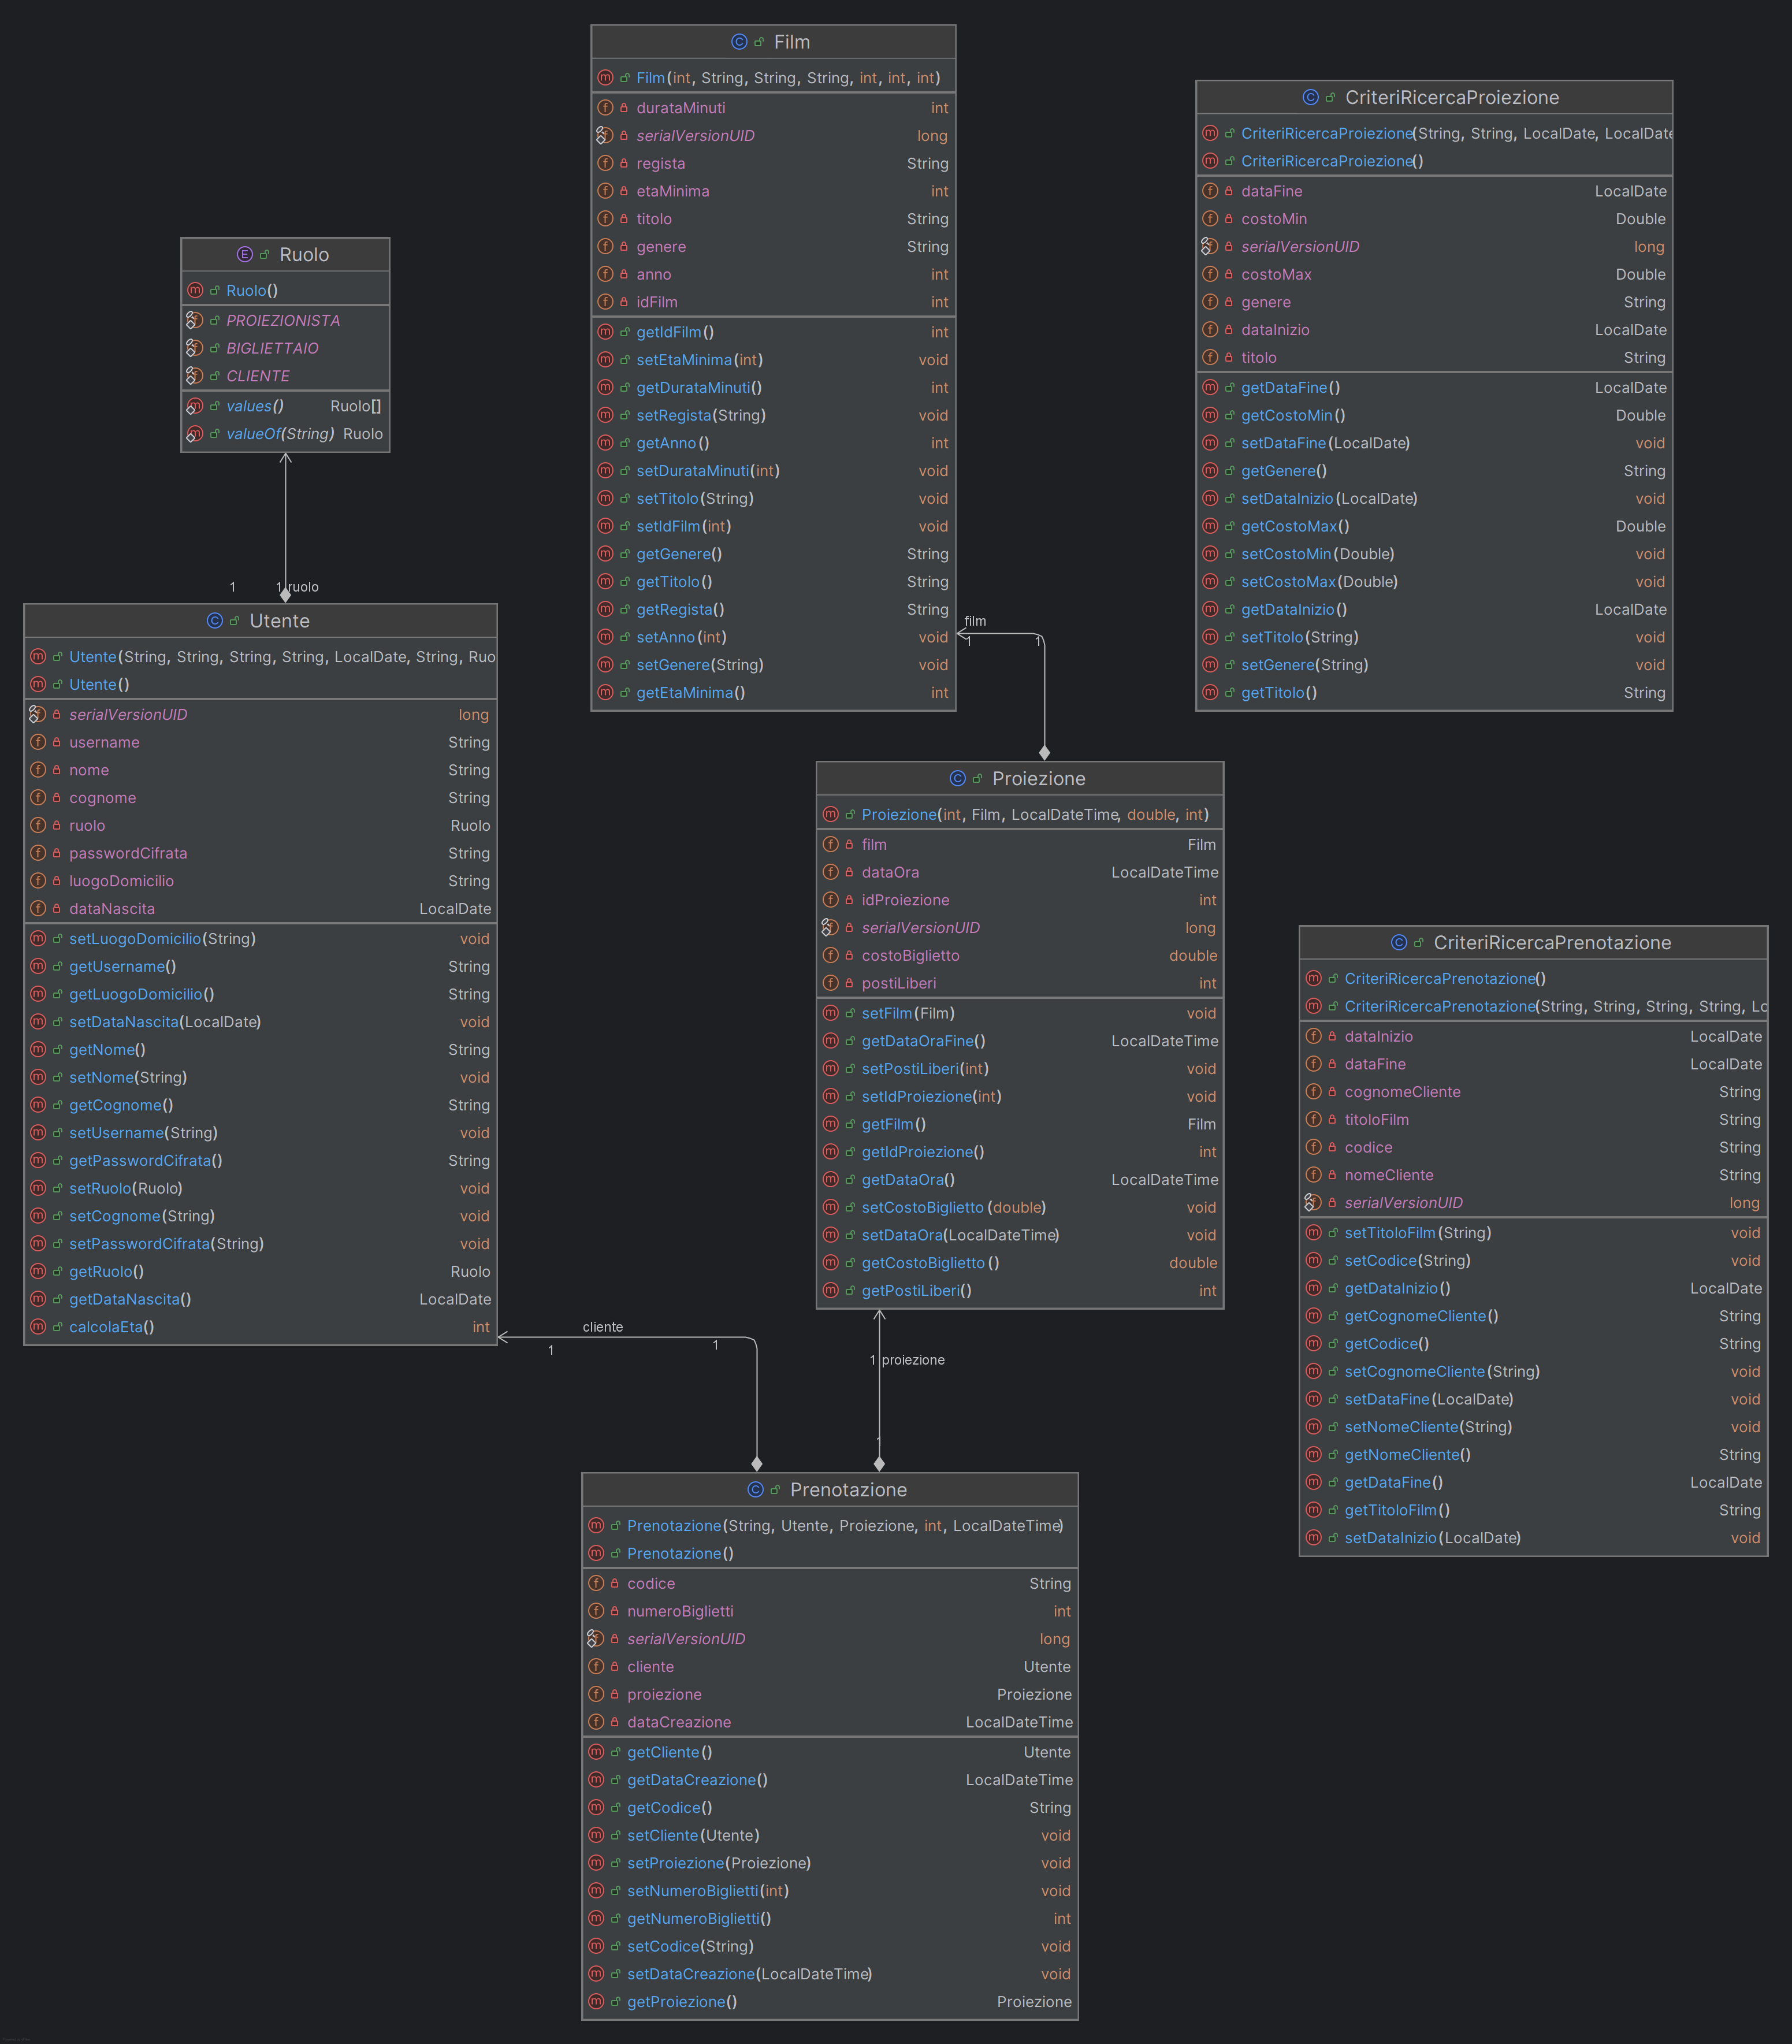
\includegraphics[width=1.0\linewidth]{DiagrammaUML.png} 
    \caption{Diagramma delle Classi UML}
    \label{fig:uml_diagram}
\end{figure}

Il diagramma sopra illustrato mostra la modellazione orientata agli oggetti delle entità di dominio presenti nel progetto nel sotto-package \texttt{common.model}. Classi fondamentali come \texttt{Utente}, \texttt{Film}, \texttt{Proiezione} e \texttt{Prenotazione} implementano l'interfaccia \texttt{Serializable} per consentire il passaggio per valore attraverso la rete. Si evidenziano attributi critici come la cifratura delle credenziali (\texttt{passwordCifrata}), la gestione delle capienze (\texttt{postiLiberi}) e i vincoli d'età delle pellicole (\texttt{etaMinima}).

Di seguito viene esposta la scomposizione analitica dei package e dei relativi componenti software:

\subsubsection{Package \texttt{cinemax.common}}
Rappresenta il punto di contatto logico e strutturale condiviso obbligatoriamente sia dal client che dal server. Contiene le interfacce remote RMI e gli oggetti di trasferimento dati (\textbf{DTO} / Model) che viaggiano sulla rete.
\begin{itemize}
    \item \textbf{\texttt{CinemaService} (Interfaccia):} Estende \texttt{java.rmi.Remote}. Dichiarerà tutti i metodi che il server si impegna ad esporre remoti (es. \texttt{autenticaUtente()}, \texttt{getPrenotazioniAttive()}, \texttt{prenotaPosto()}). Ogni metodo lancia un'eccezione controllata \texttt{RemoteException}.
    \item \textbf{Classi di Modello (\texttt{Utente}, \texttt{Film}, \texttt{Proiezione}, \texttt{Prenotazione}):} Sono classi Plain Old Java Objects (POJO) pure, implementanti l'interfaccia standard \texttt{java.io.Serializable}. La serializzazione è un requisito vincolante di Java RMI per consentire il passaggio di parametri e valori di ritorno per valore (\textit{pass-by-value}) attraverso i socket di rete, convertendo lo stato delle istanze in flussi di byte.
\end{itemize}

\subsubsection{Package \texttt{cinemax.client}}
Contiene l'infrastruttura legata alla presentazione visiva e alla cattura degli eventi.
\begin{itemize}
    \item \textbf{\texttt{ClientMain}:} Punto di ingresso dell'applicazione client; esegue la ricerca (\texttt{lookup}) nel registro RMI per ottenere il riferimento remoto dello stub di \texttt{CinemaService} e avvia l'interfaccia grafica.
    \item \textbf{Sotto-package \texttt{.view}:} Comprende le classi grafiche responsabili del layout visivo (es. \texttt{LoginFrame}, \texttt{DashboardClient}, \texttt{PalinsestoPanel}, \texttt{MappaSalaComponent}). 
    \item \textbf{Sotto-package \texttt{.controller}:} Classi mediatrici che intercettano le azioni dell'utente sulla GUI (es. la pressione di un pulsante) e invocano i metodi corrispondenti sullo stub RMI, aggiornando successivamente la vista in base alla risposta ricevuta.
\end{itemize}

\subsubsection{Package \texttt{cinemax.server}}
Contiene l'implementazione della logica di business e governa l'accesso ai servizi di backend.
\begin{itemize}
    \item \textbf{\texttt{ServerMain}:} Inizializza l'istanza del server, istanzia il registro RMI locale e vi effettua il \texttt{rebind} dell'oggetto remoto sotto una stringa identificativa univoca.
    \item \textbf{\texttt{CinemaServiceImpl}:} Estende \texttt{UnicastRemoteObject} e realizza concretamente l'interfaccia remota \texttt{CinemaService}. Al suo interno avviene il coordinamento della logica applicativa, la validazione dei vincoli aziendali e l'invocazione selettiva dei layer di persistenza.
    \item \textbf{Sotto-package \texttt{.dao} (Data Access Object):} Isola la logica di persistenza. Contiene le interfacce e le implementazioni JDBC concrete (es. \texttt{UtenteDAO}, \texttt{UtenteDAOImpl}, \texttt{ProiezioneDAOImpl}) incaricate di dialogare direttamente con il database PostgreSQL tramite query SQL native strutturate.
\end{itemize}

\subsection{Design patterns utilizzati}
Al fine di garantire flessibilità strutturale, riuso del codice e aderenza ai sani principi della programmazione orientata agli oggetti (SOLID), sono stati implementati in modo mirato i seguenti design pattern formali:

\subsubsection{Singleton Pattern (Creazionale)}
Applicato alla classe \texttt{DatabaseConnectionManager} presente nel modulo server. L'apertura e la chiusura incontrollata di connessioni di rete verso un DBMS è un'operazione computazionalmente onerosa che può portare al rapido esaurimento delle risorse del server.
\begin{itemize}
    \item \textbf{Giustificazione:} Il pattern garantisce l'esistenza di un'unica istanza centralizzata del manager di connessione per l'intera Java Virtual Machine del server. Fornisce un punto di acesso globale (\texttt{getInstance()}) e incapsula i parametri di configurazione del driver JDBC (URL, username, password), ottimizzando la gestione dei canali di comunicazione verso PostgreSQL.
\end{itemize}

\subsubsection{Data Access Object - DAO Pattern (Strutturale)}
Utilizzato capillarmente per mediare la persistenza di tutte le entità del dominio (\texttt{Utente}, \texttt{Proiezione}, \texttt{Prenotazione}, \texttt{Film}). 
\begin{itemize}
    \item \textbf{Giustificazione:} Consente di disaccoppiare radicalmente il layer della logica di business (\texttt{CinemaServiceImpl}) dal codice SQL specifico di PostgreSQL. La logica applicativa invoca metodi astratti descritti dalle interfacce (es. \texttt{proiezioneDao.findOverlappingShowtimes()}), rimanendo completamente agnostica su come i dati siano memorizzati (tabelle relazionali, file XML, database NoSQL), incrementando l'indice di manutenibilità del software.
\end{itemize}

\subsubsection{Factory Pattern (Creazionale)}
Abbinato al pattern DAO tramite la classe \texttt{DAOFactory}.
\begin{itemize}
    \item \textbf{Giustificazione:} Centralizza e scherma il processo di istanziazione dei componenti di accesso ai dati. Il server richiede le istanze dei DAO direttamente alla Factory. Se in futuro si rendesse necessario introdurre un meccanismo di caching o mutare l'implementazione concreta del DAO, sarà sufficiente intervenire sulla Factory senza alterare le classi client che ne fanno uso.
\end{itemize}

\subsubsection{Observer Pattern (Comportamentale)}
Implementato per abilitare l'aggiornamento dinamico delle interfacce grafiche a seguito di mutazioni dello stato del server (architettura basata su eventi). Nel contesto distribuito Java RMI, assume la forma di \textbf{Remote Observer Pattern}.
\begin{itemize}
    \item \textbf{Giustificazione:} Quando un cliente prenota con successo uno o più posti all'interno di una determinata proiezione, la variazione di disponibilità deve riflettersi istantaneamente sulle GUI di tutti gli altri client sintonizzati sulla medesima schermata, per prevenire tentativi di acquisto su posti ormai occupati. I client registrano un proprio stub di ascolto remoto presso il server; al verificarsi della transazione, il server itera sulla lista dei listener attivi invocando in modalità push il metodo remoto di notifica (\texttt{updateView()}), forzando il ridisegno della mappa dei posti sul client.
\end{itemize}

\subsection{Processo transazionale e concorrente di prenotazione posto}
Il flusso critico del sistema riguarda la prenotazione simultanea dello stesso identico posto (es. Riga 5, Colonna 10) per una determinata proiezione da parte di due utenti concorrenti ad un millisecondo di distanza. Per scongiurare fenomeni di \textit{overbooking} o stati inconsistenti della base dati, il flusso dinamico applica logiche di mutua esclusione sia a livello software che a livello DBMS.

Di seguito viene esposta la sequenza logica dettagliata delle operazioni (che mappa in modo speculare il relativo Diagramma di Sequenza UML):

\begin{enumerate}
    \item \textbf{Invocazione remota:} Il \texttt{ClientController} cattura l'evento di click sul posto della mappa e invoca il metodo remoto dello stub: \texttt{cinemaService.prenotaPosto(idProiezione, riga, colonna, idUtente)}.
    \item \textbf{Thread allocation:} La JVM del Server intercetta la richiesta di rete e alloca un thread dedicato dal pool RMI per servire la chiamata all'interno di \texttt{CinemaServiceImpl}.
    \item \textbf{Inizio transazione SQL:} Il server richiede una connessione al \texttt{DatabaseConnectionManager}. Al fine di controllare accuratamente le singole operazioni, disabilita il commit automatico di JDBC (\texttt{connection.setAutoCommit(false)}), avviando formalmente una transazione ACID.
    \item \textbf{Lock di lettura (Pessimistic Locking):} Il thread esegue una query SQL tramite il \texttt{PrenotazioneDAO} sul posto selezionato, sfruttando la clausola \texttt{FOR UPDATE} di PostgreSQL:
    \begin{verbatim}
    SELECT stato FROM posto WHERE id_proiezione = ? 
    AND riga = ? AND colonna = ? FOR UPDATE;
    \end{verbatim}
    Il DBMS PostgreSQL blocca la riga corrispondente nel database. Se un secondo thread concorrente tenta di verificare lo stesso posto, viene posto in stato di attesa (\textit{blocked}) finché la prima transazione non si conclude.
    \item \textbf{Verifica semantica:} Il Business Logic Tier riceve il risultato della query. Se lo stato del posto è \texttt{LIBERO}, il flusso procede. Se lo stato risulta già \texttt{OCCUPATO} (poiché il thread concorrente è arrivato un istante prima), viene sollevata un'eccezione personalizzata (\texttt{PostoGiaPrenotatoException}), la transazione esegue il \texttt{rollback} e il client riceve un messaggio di errore visivo sulla GUI.
    \item \textbf{Scrittura e generazione codice:} Il server genera un codice di prenotazione alfanumerico univoco, inserisce il record nella tabella \texttt{prenotazione} ed esegue l'update dello stato del posto a \texttt{OCCUPATO}.
    \item \textbf{Commit e Notifica dei Remote Observers:} Viene invocato il metodo \texttt{connection.commit()} per rendere permanenti e visibili le modifiche a livello globale nel database, rilasciando contestualmente il lock sulla riga. Successivamente, il server avvia un thread asincrono per scorrere la lista dei \texttt{RemoteObservers} registrati e notificare la variazione a tutti i client attivi, affinché la cella sulla mappa si colori di rosso in tempo reale.
    \item \textbf{Risposta al client:} Il metodo remoto si chiude restituendo l'oggetto \texttt{Prenotazione} serializzato al client originario, il quale mostra la schermata di conferma con il codice univoco generato.
\end{enumerate}

\subsubsection{Fase di autenticazione e login}
La fase di login descrive la transizione di stato del sistema da un utente anonimo (\textit{Ospite}) a un utente profilato e dotato di autorizzazioni specifiche basate su ruoli (RBAC).

Il diagramma di attività e sequenza per questa fase si articola nei seguenti passi essenziali:
\begin{enumerate}
    \item L'utente inserisce le proprie credenziali (\texttt{username} e \texttt{password} in testo chiaro) nei campi di testo della classe \texttt{LoginFrame} e clicca sul pulsante di accesso.
    \item Il controller del client intercetta l'action, estrae le stringhe e invoca il metodo remoto \texttt{cinemaService.autenticaUtente(username, password)}.
    \item Il server riceve le stringhe. Per ovvie ragioni di sicurezza e conformità ai principi di crittografia, le password non sono memorizzate in chiaro nel database. Il server calcola il valore di hash della password inserita utilizzando un algoritmo di hashing sicuro (es. SHA-256) combinato con una stringa di \textit{salt} univoca.
    \item Il server interroga il \texttt{UtenteDAO} passando l'username e l'hash calcolato. Il DAO esegue una query mirata sulla tabella \texttt{utente}.
    \item Se non viene trovata alcuna corrispondenza, il DAO restituisce un valore nullo; il server interpreta il risultato negativo e risponde lanciando una \texttt{CredenzialiInvalideException}, inducendo la GUI del client a mostrare una notifica pop-up di errore in rosso senza alterare lo stato della visualizzazione attuale.
    \item Se la corrispondenza ha successo, il database restituisce le informazioni anagrafiche dell'utente e il suo ruolo associato all'interno del sistema (\texttt{CLIENTE}, \texttt{PROIEZIONISTA}, \texttt{BIGLIETTAIO}).
    \item Il server istanzia un oggetto DTO di tipo \texttt{Utente}, lo popola con i dati estratti (escludendo l'hash della password per ragioni di sicurezza nel transito di rete) e lo restituisce al client.
    \item Il client riceve l'oggetto \texttt{Utente}. La classe \texttt{ClientMain} distrugge l'istanza di \texttt{LoginFrame} per liberare memoria locale e, analizzando il campo \texttt{ruolo} contenuto nel DTO, istanzia dinamicamente la specifica dashboard autorizzativa (es. abilita i menu di configurazione palinsesto solo ed esclusivamente se il ruolo corrisponde a \texttt{PROIEZIONISTA}), completando la segregazione delle responsabilità a runtime.
\end{enumerate}

\section{Progettazione della base di dati ER Relazionale} 
In questo capitolo viene dettagliato l'intero processo di progettazione, strutturazione e implementazione della base di dati relazionale a supporto del sistema \textit{CineMax}. L'obiettivo primario è definire un'architettura dei dati persistente, robusta e coerente, capace di gestire in modo efficiente le limitazioni relative agli utenti (clienti e personale), alla programmazione delle proiezioni cinematografiche e alla gestione delle prenotazioni dei posti in sala. 

Il percorso metodologico segue i canoni standard dell'ingegneria dei dati e si articola in più fasi sequenziali: si parte da un'analisi e purificazione dei requisiti per definire il dizionario dei dati, si formalizza il Modello concettuale mediante il diagramma Entità-Relazionale (ER), si analizzano le regole di business non esprimibili graficamente e si procede alla ristrutturazione dello schema eliminando i costrutti complessi. Infine, viene presentata la traduzione nel Modello logico relazionale, supportata da una verifica formale delle forme normali (BCNF/3FN) per garantire l'assenza di anomalie di aggiornamento, concludendo con le specifiche tecniche sul popolamento iniziale della base di dati tramite script dedicati.

\subsection{Analisi dei requisiti}
Il sistema \textit{CineMax} richiede la gestione persistente dei dati relativi a un'infrastruttura cinematografica. Il sistema prevede tre tipologie di utenti registrati: Clienti, Bigliettai e Proiezionisti. 
Ogni utente è identificato univocamente dal proprio username e possiede un nome, un cognome e una password. Il cinema programma una serie di proiezioni. Ogni proiezione si riferisce a uno specifico film (caratterizzato da titolo, regista, genere e durata), avviene in una determinata sala in una specifica data e ora, possiede un prezzo di biglietto e tiene traccia dei posti attualmente disponibili.
I clienti possono effettuare prenotazioni per una determinata proiezione, specificando il numero di posti desiderati. Il sistema deve garantire la coerenza dei posti della sala e impedire sovraprenotazioni.

\subsection{Modello concettuale (Diagramma ER)}
Il diagramma concettuale esprime le entità principali del sistema e le relazioni cardinali che le governano, coerentemente con i modelli definiti nel sistema:

\begin{figure}[H]
    \centering
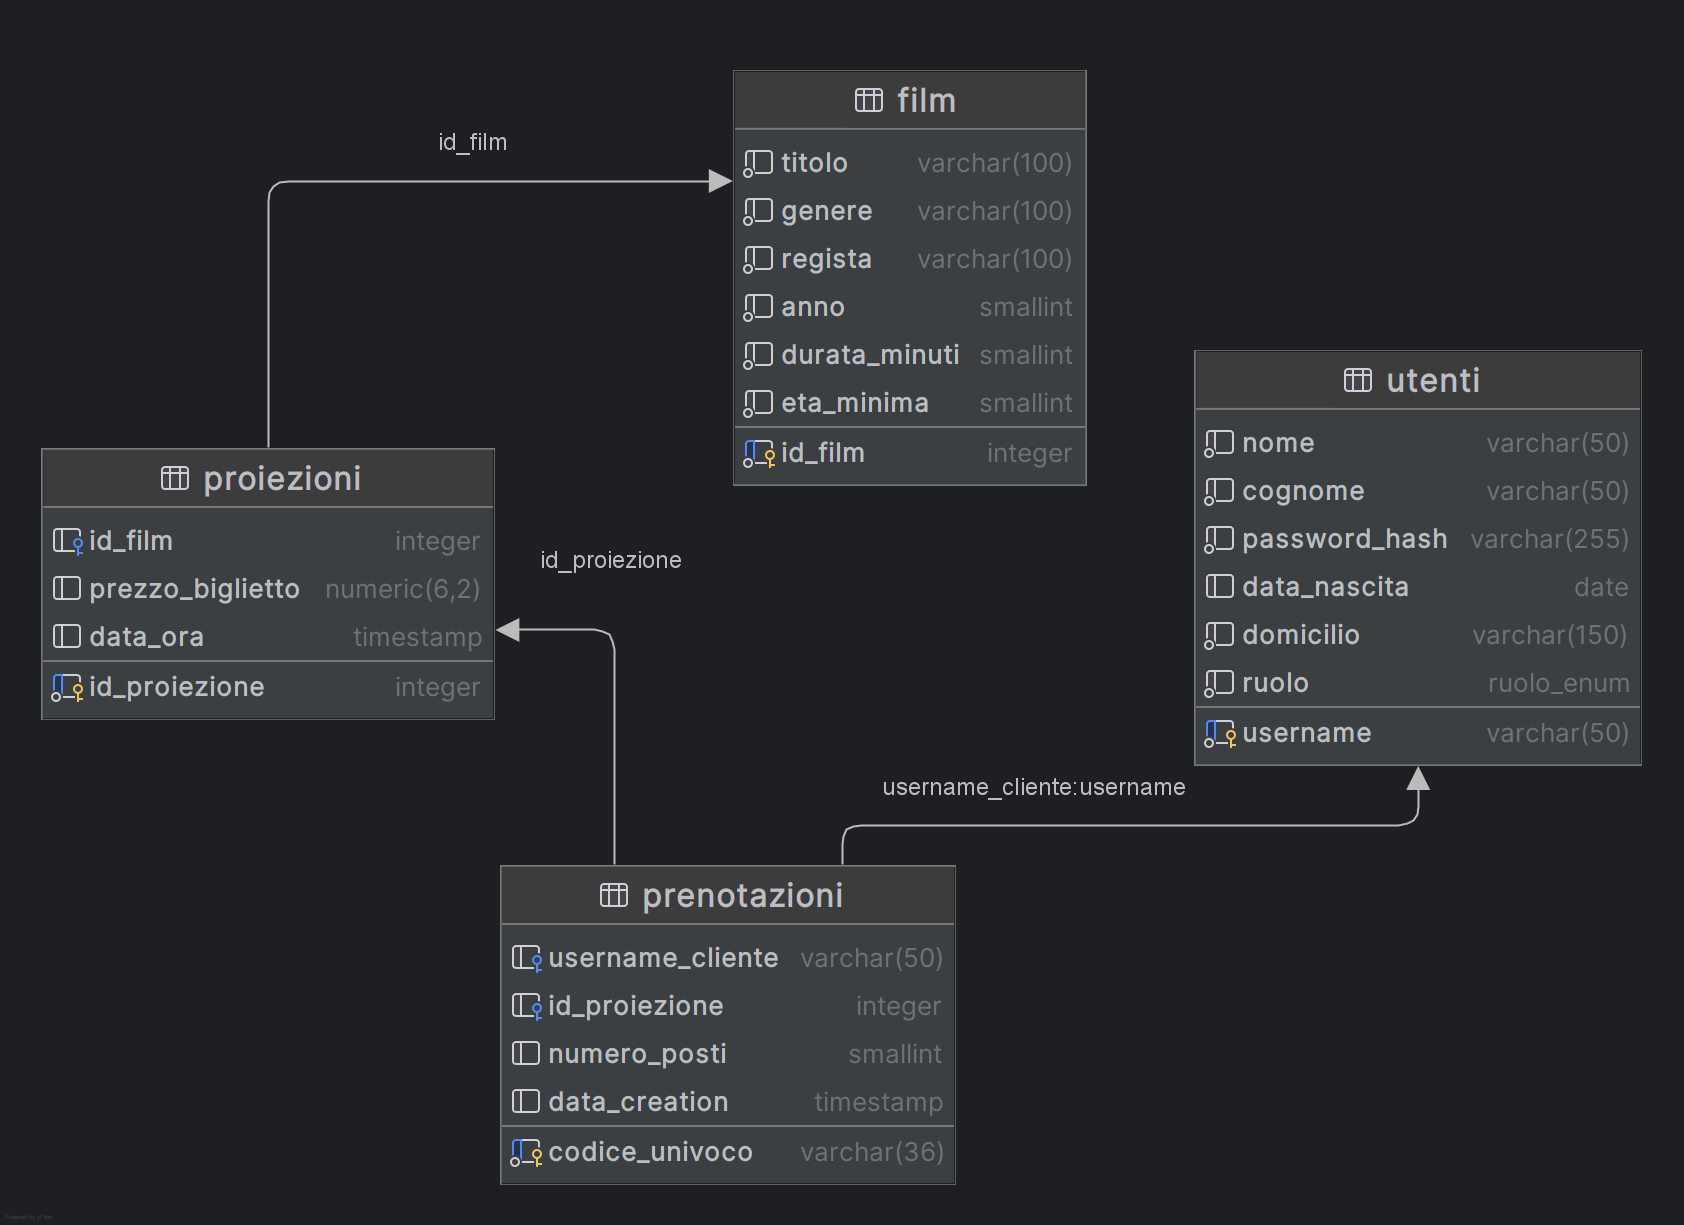
\includegraphics[width=1.0\linewidth]{DiagrammaER.png} 
    \caption{Diagramma Entità-Relazione (ER) del Database CineMax}
    \label{fig:er_diagram}
\end{figure}
\subsubsection{Specifiche delle relazioni e cardinalità}
\begin{itemize}
    \item \textbf{Effettua:} Associazione tra \textit{Utente} e \textit{Prenotazione}. Un Utente (con ruolo Cliente) può effettuare da $0$ a $N$ prenotazioni; una Prenotazione appartiene a uno e un solo Utente. (\textit{Cardinalità: 1 a N}).
    \item \textbf{Riferita a:} Associazione tra \textit{Prenotazione} e \textit{Proiezione}. Una Prenotazione è associata a una e una sola Proiezione; una Proiezione può ricevere da $0$ a $N$ prenotazioni. (\textit{Cardinalità: 1 a N}).
    \item \textbf{Caratterizza:} Associazione tra \textit{Film} e \textit{Proiezione}. Un Film può essere programmato in $0$ o più Proiezioni; una Proiezione si riferisce a uno e un solo Film. (\textit{Cardinalità: 1 a N}).
\end{itemize}

\subsection{Vincoli in linguaggio naturale}
I seguenti vincoli di integrità e regole di business non sono direttamente esprimibili mediante le notazioni standard del diagramma ER e vengono implementati a livello applicativo o tramite vincoli \texttt{CHECK} sul DBMS PostgreSQL:
\begin{enumerate}
    \item \textbf{Coerenza temporale proiezioni:} La data e l'ora di inserimento di una nuova proiezione devono essere strettamente successive alla data odierna.
    \item \textbf{Vincolo di capacità:} Il valore \texttt{num\_posti} inserito in una singola prenotazione deve essere minore o uguale ai \texttt{posti\_disponibili} della relativa proiezione al momento della transazione.
    \item \textbf{Autorizzazione ruoli (RBAC):} Solamente gli utenti aventi valore \texttt{ruolo = 'CLIENTE'} possono essere associati come intestatari di una riga nella tabella delle prenotazioni. Solamente gli utenti con \texttt{ruolo = 'PROIEZIONISTA'} possono eseguire operazioni di inserimento o modifica sulle proiezioni.
    \item \textbf{Unicità di sala:} Non possono essere programmate due proiezioni nella stessa sala alla stessa data la cui distanza temporale sia inferiore alla durata del film associato alla prima proiezione aumentata di un intervallo di pulizia della sala standard (30 minuti).
\end{enumerate}

\subsection{Ristrutturazione dello schema ER}

\subsubsection{Eliminazione di attributi composti o multivalore}
\begin{itemize}
    \item \textbf{Ruolo:} L'attributo ruolo dell'utente è modellato come un tipo enumerativo atomico (\texttt{Ruolo}), garantendo l'assenza di strutture composte direttamente all'interno dell'entità.
    \item \textbf{Dati anagrafici:} Nome e cognome sono stati separati fin dal principio come attributi atomici testuali distinti per evitare stringhe composte difficili da indicizzare e manipolare.
\end{itemize}

\subsubsection{Analisi delle ridondanze}
\begin{itemize}
    \item \textbf{Attributo \texttt{posti\_disponibili} in \textit{Proiezione}:} Dal punto di vista puramente teorico, questo attributo rappresenta una ridondanza, in quanto il numero di posti disponibili potrebbe essere calcolato dinamicamente a runtime effettuando una sottrazione tra la capacità nominale della sala (200 posti) e la sommatoria (\texttt{SUM}) dell'attributo \texttt{num\_posti} di tutte le prenotazioni associate a quella specifica proiezione.
    \item \textbf{Motivazione del mantenimento:} Si è scelto formalmente di \textbf{mantenere la ridondanza} per ragioni di ottimizzazione prestazionale delle query di lettura frequenti sulla dashboard del client, diminuendo il carico computazionale sul DBMS ed evitando join onerosi sul calcolo in tempo reale.
\end{itemize}

\subsection{Modello Logico Relazionale}
Si procede alla traduzione dello schema E-R ristrutturato nel modello logico relazionale. Le chiavi primarie sono indicate in sottolineato, mentre le chiavi esterne sono contrassegnate dalla sigla FK.

\begin{itemize}
    \item \textbf{UTENTI} (\underline{username}, nome, cognome, password\_hash, data\_nascita, domicilio, ruolo)
    \item \textbf{FILM} (\underline{id\_film}, titolo, genere, regista, anno, durata\_minuti, eta\_minima)
    \item \textbf{PROIEZIONI} (\underline{id\_proiezione}, data\_ora, \textit{id\_film}, prezzo\_biglietto)
    \item \textbf{PRENOTAZIONI} (\underline{codice\_univoco}, \textit{username\_cliente}, \textit{id\_proiezione}, numero\_posti, data\_creazione)
\end{itemize}

\subsection{Analisi delle Dipendenze Funzionali e Normalizzazione}
Al fine di garantire l'assenza di anomalie di inserimento, cancellazione e aggiornamento, le relazioni strutturate sono state sottoposte a verifica formale rispetto alla \textbf{Terza Forma Normale (3FN)} e alla \textbf{Forma Normale di Boyce-Codd (BCNF)}.

Prendendo in esame la relazione \textbf{UTENTI}:
\begin{equation*}
    \text{username} \rightarrow \text{nome, cognome, password\_hash, data\_nascita, domicilio, ruolo}
\end{equation*}
L'unica dipendenza funzionale ha come determinante la chiave primaria (\texttt{username}), che è superchiave. Non esistono dipendenze transitive tra attributi non chiave. Pertanto, la relazione soddisfa pienamente i requisiti della BCNF. Lo stesso principio di scomposizione atomica è stato applicato alle restanti tabelle, garantendo che ogni determinante sia una superchiave.

\subsection{Script DDL di Creazione del Database (PostgreSQL)}
Di seguito si riporta lo script SQL nativo per la generazione delle tabelle e l'applicazione dei vincoli di integrità referenziale e semantica all'interno del RDBMS:

\begin{lstlisting}[language=SQL, basicstyle=\small\ttfamily, frame=single, breaklines=true, postbreak=\mbox{\textcolor{red}{$\hookrightarrow$}\space}]
-- Creazione del tipo enumerativo richiesto dalla tabella utenti
CREATE TYPE ruolo_enum AS ENUM ('CLIENTE', 'BIGLIETTAIO', 'PROIEZIONISTA');

CREATE TABLE utenti (
    username         VARCHAR(50)   PRIMARY KEY,
    nome             VARCHAR(50)   NOT NULL,
    cognome          VARCHAR(50)   NOT NULL,
    password_hash    VARCHAR(255)  NOT NULL,
    data_nascita     DATE,
    domicilio        VARCHAR(150)  NOT NULL,
    ruolo            ruolo_enum    NOT NULL
);

CREATE TABLE film (
    id_film          SERIAL        PRIMARY KEY,
    titolo           VARCHAR(100)  NOT NULL,
    genere           VARCHAR(100)  NOT NULL,
    regista          VARCHAR(100)  NOT NULL,
    anno             SMALLINT      NOT NULL CHECK (anno BETWEEN 1888 AND 2100),
    durata_minuti    SMALLINT      NOT NULL CHECK (durata_minuti > 0),
    eta_minima       SMALLINT      NOT NULL DEFAULT 0 CHECK (eta_minima >= 0)
);

CREATE TABLE proiezioni (
    id_proiezione    SERIAL        PRIMARY KEY,
    data_ora         TIMESTAMP     NOT NULL,
    id_film          INT           NOT NULL REFERENCES film(id_film) ON DELETE CASCADE,
    prezzo_biglietto NUMERIC(6,2)  NOT NULL CHECK (prezzo_biglietto >= 0)
);

CREATE TABLE prenotazioni (
    codice_univoco      VARCHAR(36)  PRIMARY KEY,
    username_cliente    VARCHAR(50)  NOT NULL REFERENCES utenti(username) ON DELETE CASCADE,
    id_proiezione       INT          NOT NULL REFERENCES proiezioni(id_proiezione) ON DELETE CASCADE,
    numero_posti        SMALLINT     NOT NULL CHECK (numero_posti > 0),
    data_creazione      TIMESTAMP    NOT NULL DEFAULT NOW()
);
\end{lstlisting}

\section{Sitografia e bibliografia}
\begin{itemize}
    \item Oracle Java Documentation \url {https://docs.oracle.com/en/java/}
    \item Apache Maven Project \url{https://maven.apache.org/}
    \item PostgreSQL Official Documentation: \url{https://www.postgresql.org/docs/}
\end{itemize}
\end{document}\begin{figure}
    \centering
    \includegraphics[width=0.5\linewidth]{Oracle.png}
    \caption{Enter Caption}
\begin{figure}
        \centering
        \includegraphics[width=0.5\linewidth]{apachemaven.png}
        \caption{Enter Caption}
        \label{fig:placeholder}
    \end{figure}
        \label{fig:placeholder}
\end{figure}
